\chapter{Volatility}\label{chap:volatility}			
In statistical terms the study of financial volatility is a scale problem. It is concerned with the fluctuation of price about a particular direction of movement rather than the direction itself. For most purposes the location component of the statistical problem can be ignored.  In its most common usage, volatility refers to the standard deviation of the change in the log-price of an asset over some fixed period of time (although in the financial literature, volatility may also refer to the variance). Individual volatilities also play an important role when considering correlations between different assets. 

We will see that there are two main approaches to volatility and covolatility estimation. One is built around the concept of `stochastic volatility' where volatility is viewed as a latent unobserved stochastic process. The other is centred on `time-change' where volatility is considered to be constant on an alternative non-physical time scale. Both approaches enable the cumulative volatility  to be estimated over a given interval of physical time.  

In this chapter and the next, we look back at two remarkable papers by Zhou (1995,1996). This is partly to emphasise their historical importance in the early development of the subject but also to show they provide common ground for the two main estimation approaches described above.  Additionally by developing a systematic method of proof for the theorems in \citet{zhou1996high} we are able to show that Zhou's methods can provide an `infill consistent' estimator of cumulative volatility as conjectured by \citet{hansen2006realized}, albeit under rather strong conditions on the infill observation times. 

There is an extensive literature on volatility and covolatility in financial mathematics and econometrics. \citet{mcaleer2008realized} and \citet{ait2009estimating} provide substantial reviews. The recently published compendium edited by \citet{bauwens2012handbook} has contributions from 39 authors, with almost 1000 references. 

Although the practicalities of high-frequency trading favour the time-change approach, we outline key results in modern stochastic volatility theory and indicate conditions under which powerful asymptotic results have been obtained. We start by describing the standard model framework for inference, outlining key results and defining a basic class of volatility estimators.  We explain the use of the \emph{signature plot} as a graphical diagnostic but argue that the variogram provides a more natural plot providing greater insight. Various volatility estimators that have been proposed in the literature are shown to be equivalent to simple summaries of the empirical variogram. 

The time-change approach opens up the possibility of using classical Kalman filtering methods in the Dynamic Linear Model framework. These techniques are illustrated in Section \ref{sec:timedependency}. We then consider criticisms that have been levied at the standard model. A Monte Carlo goodness of fit test for the model is proposed and its significance is assessed for financial data.  Finally we apply our modified volatility estimator to the problem of estimating daily patterns of volatility in the US Dollar -- Japanese Yen exchange rate.
 
\section{Latent price -- physical time}
There is a long tradition in mathematical finance of using continuous time models for describing the behaviour of asset returns. Empirical evidence shows that logarithmic returns on equities, currencies and commodities can be approximately modelled as normal mixtures with varying standard deviations. For a detailed discussion with application to the movement of foreign exchange rates, see \citet{dacorogna2001introduction}.

Much of the theoretical work on volatility problems is carried out in the framework of stochastic differential equations (SDEs) and It\^{o} calculus. 
A basic and traditional model for the latent `efficient' log-price,  $\breve{X}(t)$, of a financial asset is 
\begin{equation}\label{eq:model1} d\breve{X}(t) = \sigma(t) dB(t),\end{equation}
where $B(t)$ is standard Brownian motion and the infinitesimal standard deviation $\sigma(t)$ is either deterministic or stochastic. The value $\sigma(t)$ is also called the \emph{instantaneous volatility} at time $t$. Usually $t$ represents ordinary physical time -- sometimes termed `wall-clock' time. Various models for the stochastic evolution of $\sigma(s)$ have been proposed; predominant among these are the ARCH class of models and related generalisations. For a wide historical review of the mathematical modelling of financial time series, see \citep{shephard2015martingale}. 

Note that the stochastic differential equation above has no drift term. This is in accordance with a fundamental principle of mathematical finance, the martingale property in which the current log-price is supposed to incorporate all available information and hence represent the consensus  prediction of expected log-price going forward, at least in the short term. The minimal assumption of no arbitrage in the price process leads, under some regularity conditions, to the consequence that the price process is a semi-martingale; see Delbaen and Schachermayer (1994). 



\subsection{Realised volatility}
Suppose $\breve{X}_1$ is the latent efficient log-price at time $t_1$ and $\breve{X}_2$ is the value at time $t_2$.  The change in value, $\breve{X}_2-\breve{X}_1$ is called the \emph{return} or \emph{log-return} over the \emph{return period} $(t_1,t_2)$. 
In the above model \eqref{eq:model1}, the return over a unit of time $(0,1)$ has mean zero and variance 
\begin{equation}\label{eq:volT}
v = \text{Var}[\breve{X}(1) - \breve{X}(0)] = \int_0^1 \sigma^2(s) ds,
\end{equation}
conditional on $\sigma$.

The \emph{theoretical volatility} over $(0,1)$ is the square root of this quantity. Using the additive property of variances for processes with conditionally independent increments (conditional on $\sigma$), the theoretical volatility \eqref{eq:volT} can be written as 
$$
\sum_{i=1}^n \int^{t_i}_{t_{i-1}} \sigma^2(s)ds = \sum_{i=1}^n \EE(R_i^2),$$
where $R_i = \breve{X}_i - \breve{X}_{i-1}$ is the return over the sub-interval $(t_i, t_{i-1})$ and $(t_i, i = 0,1,\dots,n)$ is an increasing sequence of times  with $t_0 =0$ and $t_n = 1$.  

Assuming that the returns $\{R_i = r_i\}$ are observable, $\sum_{i=1}^n r_i^2$ is an obvious estimate of $v$. With observations $x_i = x(t_i)$ at $t_i, i=0,\dots,n$, the statistic
$$ \hat{v}(x) = \sum_{i=1}^n (x_i - x_{i-1})^2,$$
is called the \emph{realised variance} of $x$ over $(0,1)$. 
The \emph{realised volatility} $\text{RVol}(x)$ is the square root of $\hat{v}(x)$ but note again the confusion between variance and volatility in the financial terminology. 
 
The basic philosophy of financial mathematics is there is hidden latent efficient price $\bX$
which is not observable directly. \citet{merton1980estimating} noticed that if the hypothetical values of $\breve{X}$ are available on an arbitrarily fine time scale, $v$ can be recovered with arbitrary precision, under the model in (\ref{eq:model1}). Subsequently \citet{andersen2001distribution}, \citet{barndorff2002econometric} and \citet{mykland2006anova} among others, show this rigorously by considering the realised variance $$\hat{v}(\breve{X};n) = \sum_{i=1}^n \left(\breve{X}(t_i^{(n)}) - \breve{X}(t_{i-1}^{(n)})\right)^2
$$ for a sequence of partitions $(t^{(n)}_0 = 0, t^{(n)}_1,\dots,t^{(n)}_n = 1)$ where $\max_i|t^{(n)}_i - t^{(n)}_{i-1}| \to 0$ as $n \to \infty$.  

Furthermore \citet{barndorff2002econometric}, under quite general conditions, show that $\hat{v}(\breve{X};n)$ is asymptotically normally distributed.  In their analysis, the instantaneous volatility is assumed to have locally square integrable sample paths, while being stationary and stochastically independent of the Brownian motion $B(t)$, and most importantly, it assumed that the latent efficient price is available.  
Taking $t^{(n)}_i = i\Delta, i=0,\dots,n$, $\Delta = n^{-1}$, they show
\begin{equation}\label{eq:BNasympt}
\Delta^{-1/2} \frac{\hat{v}(\breve{X};n) - \int_0^1 \sigma^2(s) ds}{\sqrt{2 \int^1_0 \sigma^4(s)ds}} \to N(0,1),
\end{equation}
as $\Delta \to 0$. 

This type of result is called \emph{infill asymptotics} -- corresponding to an increasingly high frequency of observations within an interval of fixed total length. Here $\Delta^{-1}$ plays the r\^{o}le of $n$ in the traditional area of asymptotic statistical analysis.

In a series of paper reported in \citet{barndorff2004power} and the references therein, the authors introduce the \emph{bipower} estimate of integrated variance, namely 
$$\hat{v}^{[1,1]}(x;n) = \sum_{i=1}^{n-1} \left|x(t_i^{(n)}) - x(t_{i-1}^{(n)})\right|\left|x(t_{i+1}^{(n)}) - x(t_{i}^{(n)})\right|.
$$
The estimator, $\hat{v}^{[1,1]}(\breve{X};n)$, is shown to be robust to additional jump terms in the model specification of the latent log-price process $\breve{X}$ and hence by comparison with the realised variance they are able to detect and quantify the contributions of jumps in latent log-price volatility.  

\citet[Section 5.4]{barndorff2004power}  report that, jointly,
$$ \frac{\Delta^{-1/2}}{\sqrt{\int_0^1\sigma^4(u)du}} \begin{pmatrix} \hat{v}(\breve{X};n) - v \\ \hat{v}^{[1,1]}(\breve{X};n) - v \end{pmatrix} 
\to N\left\{ 0,\begin{pmatrix} 2 & 2 \\ 2 & 2.60907 \end{pmatrix}\right\},
$$ 
as $\Delta \to 0$, under the conditions of \eqref{eq:BNasympt}. These results show how much statistical information is lost in using the bipower estimator with latent log-prices. 

\paragraph{Annualised volatility}
In the financial world, daily realised volatility, $\text{RVol}_\text{Day}(x)$, is usually extrapolated to give an estimate of yearly volatility, by assuming additivity for variances.   The extrapolated figure is then multiplied by 100 and reported as a percentage. So with a nominal 252 trading days in the year, the annualised volatility is
$$ \text{RVol}_{\text{Annual}} \approx 100 \sqrt{252} \; \text{RVol}_{\text{Day}}(x)\%.$$

\subsection{Signature plots and variograms} 
It is tempting to conclude that the log-price process should be sampled at the highest frequency to produce the best estimate of $v$. 
As a check it is helpful to plot $\hat{v}_n$ for various values of the sampling interval, $\Delta$. The resulting graph is called a \emph{signature plot} \citep{andersen2000great}. Typically the curve is not flat, as would be predicted by the model in (\ref{eq:model1}). Very often the curve increases as the $\Delta$ becomes small and the sampling frequency increases, see Figure \ref{SignaturePlot}.
\begin{figure}[!ht]
\centering
%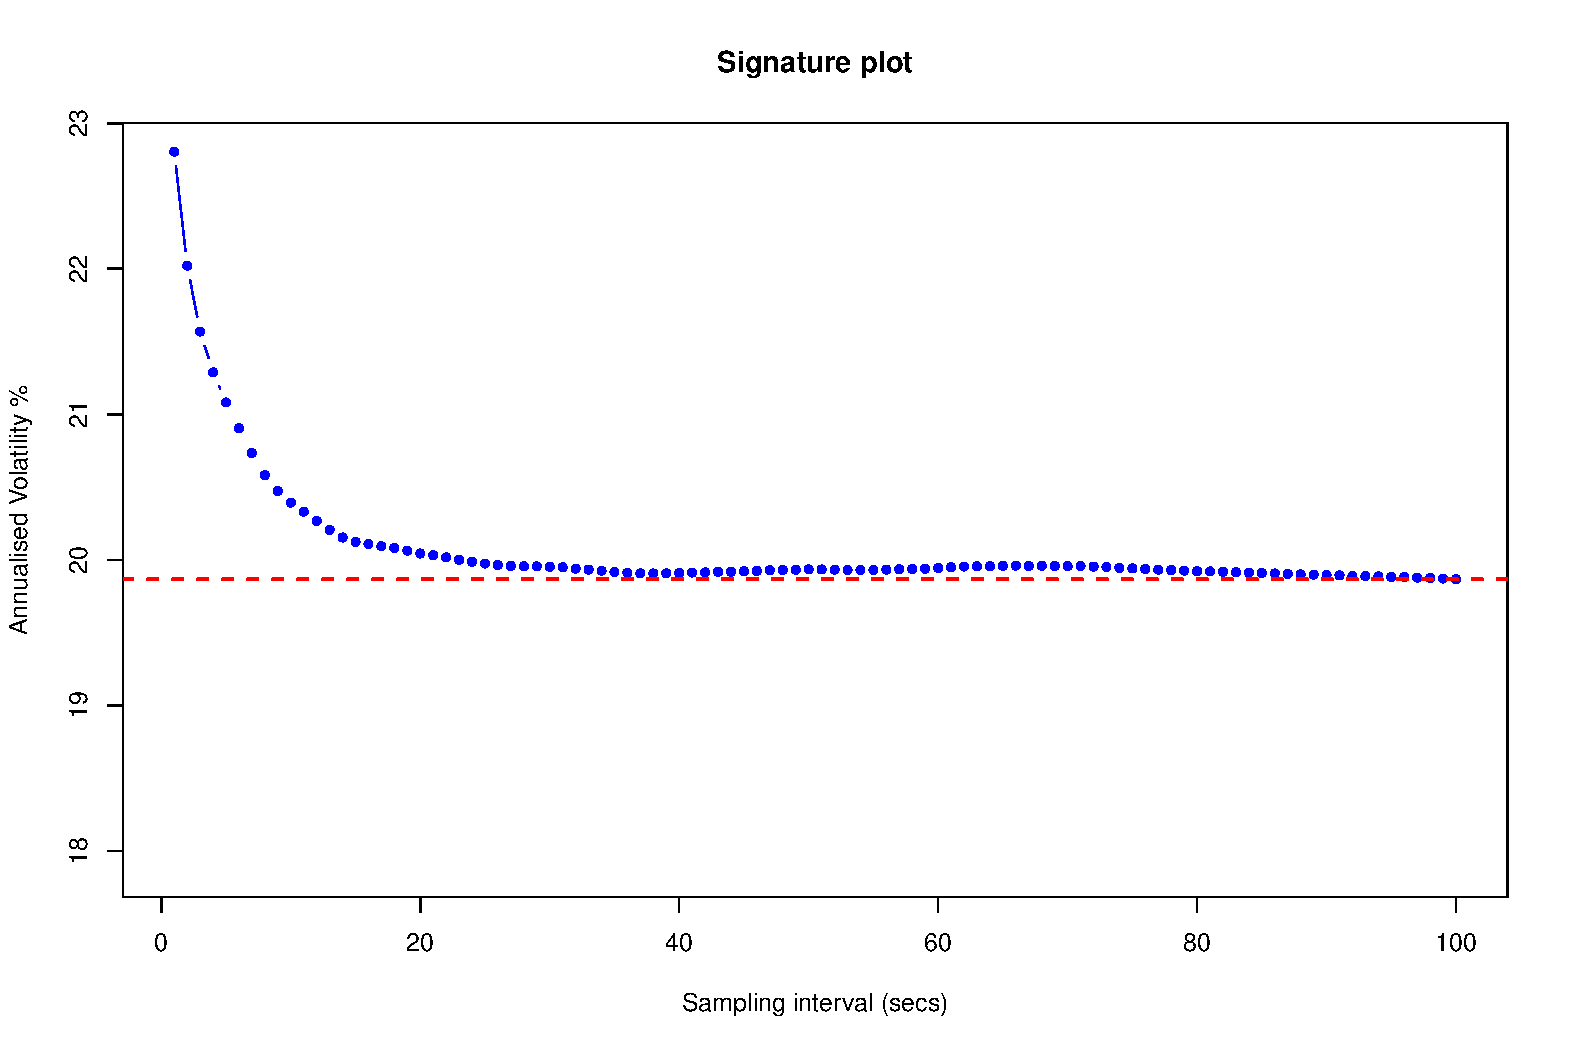
\includegraphics[width=\linewidth]{./Figures/SingleSignaturePlot.pdf}
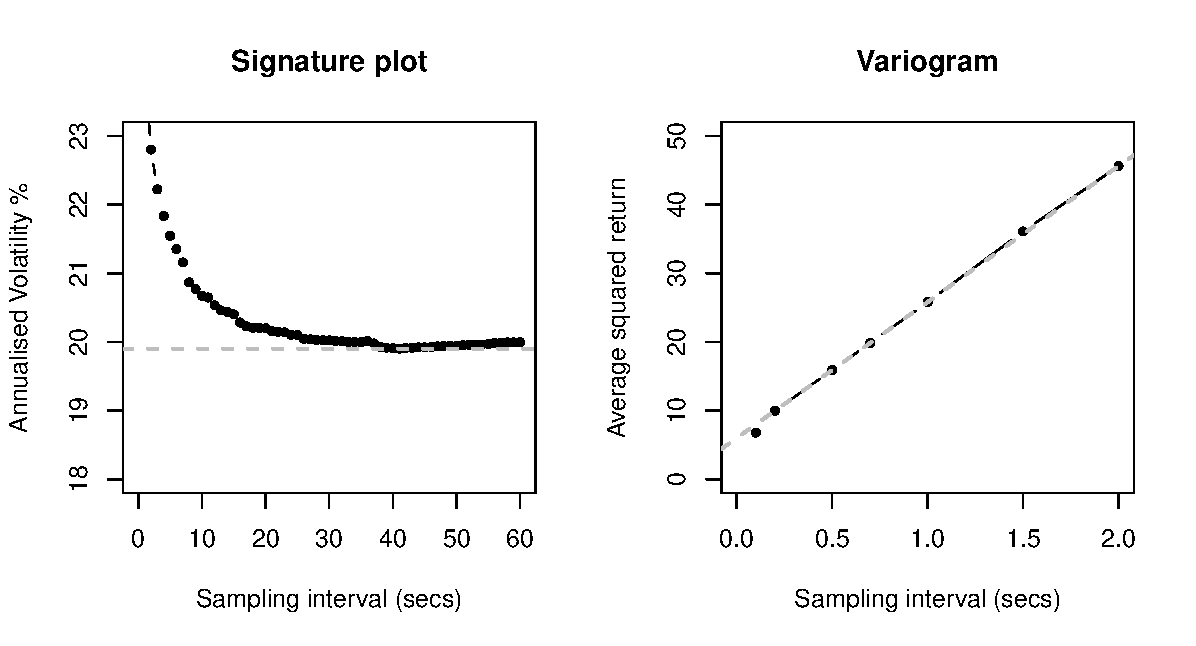
\includegraphics[width=\linewidth]{./Figures/chap4SigVol.pdf}
\caption{Signature and variogram plot: USD/EUR trade data 2008-10-09 (EBS)\label{SignaturePlot} }
\end{figure}

The variogram plot is an alternative way of showing the relationship between volatility and sampling frequency.  It is used extensively in geostatistics \citep{cressie1993statistics}. The theoretical variogram of a one-dimensional process $X$ with stationary increments is defined to be
$$ \Gamma(\tau) = \EE{[X(t+\tau) - X(t)]^2},\quad \tau > 0.$$  It can be estimated by
$$\hat{\Gamma}(\tau) = \frac{\sum_{(i,k) \in M(\tau)}[x(t_i) - x(t_k)]^2}{|M(\tau)|},\quad \tau > 0,$$
where $M(\tau)$ is the set of pairs $(i,k)$ such that $t_k = t_i + \tau$ and $|M(\tau)|$ is the cardinality of $M(\tau)$. In practice, it may not be possible to find points $(t_i,t_k)$ that are exactly separated by $\tau$, in which case a certain tolerance is allowed in defining $M(\tau)$.
Figure \ref{SignaturePlot} compares the estimated variogram with the signature plot. Note that in this case the variogram is approximately linear with a positive intercept. For discussion of the use of variograms in volatility estimation with an illustration, see Section \ref{sec:variogram}.
%  

\section{Observed price -- physical time}
In an early paper, \citet{roll1984simple} suggested that observations of the process in (\ref{eq:model1}) should be modified by the introduction of a random  error term. Roll was motivated by problems in dealing with trade data when there is no information about whether the trade is from the bid or the ask side of the order book. In its simplest form the revised model for observations at times $\{t_i\}$  is  
\begin{equation}\label{eq:model2} X_i = \breve{X}_i + \epsilon_i, \quad i \in \mathbb{Z}, \end{equation}
where $\breve{X}_i = \breve{X}(t_i)$ is the latent efficient log-price,  $X_i = X(t_i)$ is the observed value, and  $\{\epsilon_i\}$ are iid with constant variance $\eta^2$.  The model has become widely accepted in mathematical finance as a suitable framework for volatility analysis. In this model the efficient price $\bX(t_i)$
cannot be observed and the observed price $X(t_i)$is the
efficient price plus perturbations. The perturbations $\{\epsilon_i\}$ are often termed \emph{microstructure noise}. 

With $X$ given by (\ref{eq:model2}), the realised variance is no longer an unbiased estimator of the integrated variance $v_T$. This noise component produces an inflated effect that makes the
volatility more than what it should be. Assuming equally spaced sampling with $\Delta = 1/n$, it follows that
\begin{equation}\label{eq:Qbias} \EE \hat{v}(X) = \frac{2\eta^2}\Delta  +  \int_0^1 \sigma^2(s) ds = \frac{2\eta^2}\Delta  + v.\end{equation}
There is a discontinuity as $\Delta \to 0$, in qualitative agreement with observed signature plots (Figure \ref{SignaturePlot}). Similarly, the variogram estimator has approximate expectation 
\begin{equation} \label{eq:variogramexp} \EE \hat{\Gamma}(\Delta) \approx 2\eta^2 + \Delta \int_0^1 \sigma^2(s) ds,\end{equation}
for small $\Delta$, i.e.\ linear with slope equal to the integrated variance $\int_0^1 \sigma^2(s) ds$ and intercept twice the microstructure variance -- again in agreement with observation (Figure \ref{SignaturePlot})

There is an extensive literature on methods of improving the estimator $\hat{v}(X)$ in the context of model \ref{eq:model2}.  As noted in Section 4.1.1, when the underlying efficient price is observable then its volatility can
be obtained with arbitrary precision using data observed on an arbitrary high-frequency
timescale. However historically, as prices started to be observed with increasingly high frequency, it was noticed that microstructure noise
became dominant. So instead of providing increased accuracy the realised volatility became more and more biased.
Compromises were made to observe the price over time intervals
such as 1 minutes or 1 second. A basic understanding of these compromises is contained in an early paper by \citet{zhou1996high}, submitted to the Journal of Business \& Economic Statistics in 1993, over 20 years ago. These ideas are discussed in the next section.
%
%
\subsection{Zhou's contribution}
\citet{zhou1996high} describes his experiences in working with tick-by-tick data in foreign exchange trading where a succession of proposed exchange rates are seen at irregular times on the Reuters news feed.   He observed that successive returns of these prices over short periods of time are highly negatively correlated. For trade data this might be explained by the bid-ask bounce phenomenon illustrated in Figure \ref{fig:OBbounce}.  However, Zhou found similarly large negative correlation when using the bid price alone. He then proposed model  (\ref{eq:model2}) as an explanation. He showed how to estimate the underlying volatility unbiasedly, stated the variance of his estimator and indicated how this result could be obtained. 

Zhou's estimator for the integrated variance, $v = \int_0^1 \sigma^2(s) ds$, is
\begin{equation}\label{eq:Zhou1} G = \sum_{i=1}^n R_{i,1} R_{i+1,3},
\end{equation}
where $R_{i,k} = X_i - X_{i-k}$, the return over the period $(t_{i-k}, t_i)$.  Zhou's key observation is that the error terms in 
\begin{align}\label{eq:R1}
R_{i,1} &= \breve{X}_i - \breve{X}_{i-1} + \epsilon_{i} - \epsilon_{i-1}  \\
R_{i+1,3} &=\breve{X}_{i+1} - \breve{X}_{i-2} + \epsilon_{i+1} - \epsilon_{i-2},\nonumber
\end{align} 
are independent, and since $R_{i+1,3}$ can be written as a sum of independent increments 
\begin{equation} \label{eq:R3} R_{i+1,3} =\breve{X}_{i+1} - \breve{X}_{i} + \breve{X}_{i}- \breve{X}_{i-1} + \breve{X}_{i-1} - \breve{X}_{i-2} + \epsilon_{i+1} - \epsilon_{i-2}
\end{equation} then
\begin{equation}\label{eq:sigmai} \EE R_{i,1} R_{i+1,3} = \EE (\breve{X}_{i-1} - \breve{X}_{i})^2  = \int_{t_{i-1}}^{t_i} \sigma^2(s) ds \overset{\text{defn}}{=} v_i^2.
\end{equation}
Taking $t_0 = 0$ and $t_n = 1$, it follows that $G$ is an unbiased estimator of $v = \int_0^1 \sigma^2(s) ds.$ Zhou is the first person to suggest the estimator $G$. .

As pointed out by Zhou, the variance of $G$ is complicated for arbitrary non-constant $\{v_i\}$, and Zhou does not derive an expression for the variance in the general case.  We derive the general variance  in Theorem \ref{thm:inhomogzhou}.  

However by assuming that $v_i = v/n, i=1,2,\dots,n$, Zhou obtains the following.
\begin{thm}[Zhou, 1996]\label{thm:zhou1}
Let $\breve{X}_i - \breve{X}_{i-1} \sim N(0,v/n)$ and $\epsilon_i \sim N(0,\eta^2)$, independently $i \in \mathbb{Z}$, then
\begin{equation}\label{eq:zhou1a} \VV G = \frac{v^2}{n^2} (6n -2) + 8 v \eta^2 + (8n -6) \eta^4.\end{equation}
\end{thm}
%
%
\noindent \emph{Remark.} There is a typographical error in Zhou's statement of the theorem, corrected above -- the coefficient in last term should be $(8n -6)$ not $(8n-4)$. Zhou indicates a method of proof without full details. To obtain the result it is necessary to assume that the random variables are normally distributed or at least have zero kurtosis.  The method of proof we develop below will be helpful in later parts of this chapter. 

Although the assumption of constant $\{v_i\}$ seems restrictive, it will be applicable when working on volatility stabilising activity-timescale, for example, when observing prices at transaction times. See the discussion in Section \ref{sec:timedependency}.  

We start by proving the theorem under Zhou's conditions and derive a more general version later in Theorem \ref{thm:inhomogzhou}.  
\begin{proof}
Let $Z = (Z_1,\dots,Z_{2n+6})\tz$ be a vector of iid $N(0,1)$ variables, then from (\ref{eq:R1}) and (\ref{eq:R3}), we see that $G$ has the same distribution as the quadratic form 
\begin{equation}\label{eq:QF} Z\tz [\alpha I_R: \eta J_R]\tz [\alpha I_S: \eta J_S] Z,
\end{equation}
where $\alpha= \surd(v/n)$ and 
$I_R, J_R, I_S$ and $J_S$ are $n \times (n+3)$ dimensional Toeplitz matrices with first rows given respectively by
\begin{align}\label{eq:toeplitz}
\text{Row 1: } &I_R = (0,0,1,0,\dots,0) \nonumber \\
\text{Row 1: } &J_R = (0,-1,1,0,\dots,0)\nonumber\\
\text{Row 1: } &I_S = (0,1,1,1,0,\dots,0) \nonumber\\
\text{Row 1: } &J_S = (-1,0,0,1,0,\dots,0) 
\end{align}
The remaining elements in their first columns are zero. 

From standard multivariate normal theory \citep{rencher2012methods}, we have
$$ \EE Z\tz H Z = \text{trace} H \quad \text{and} \quad \VV Z\tz H Z = 2 \text{ trace} \left\{ \left(\frac{H+ H\tz}{2}\right)^2\right\}.$$ 
In our case 
$$ H = \begin{pmatrix} \alpha^2 I_R\tz I_S & \alpha \eta I_R\tz J_S\\ \alpha \eta J_R\tz I_S & \eta^2 J_R\tz J_S  \end{pmatrix},$$
so that 
\begin{align*}\EE G = \text{trace} H &= \alpha^2 \text{ trace } I_R\tz I_S + \eta^2 \text{ trace } J_R\tz J_S\\
&= \alpha^2 n + 0 = \frac{v}{n} n = v.
\end{align*}

For an arbitrary symmetric square matrix
$$\label{eq:traceVar}  \text{trace } A^2 = \sum_i \sum_j A_{ij}^2 = ||A||^2_2.$$

The variance of $G$ is then
\begin{equation}\label{eq:zhouVar}
\VV G = \frac12 \alpha^4 ||I_R\tz I_S + I_S\tz I_R||^2_2 + \alpha^2\eta^2 || I_R\tz J_S + I_S\tz J_R||^2_2 + \frac12 \eta^4||J_R\tz J_S + J_S\tz J_R||^2_2.
\end{equation}
Inspecting the pattern of these matrix products we have, by induction, 
\begin{align*}
||I_R\tz I_S + I_S\tz I_R||^2_2 &= 12n-4\\
|| I_R\tz J_S + I_S\tz J_R||^2_2 &= 8n\\
||J_R\tz J_S + J_S\tz J_R||^2_2 &=16n -12.
\end{align*}
Substituting these values in (\ref{eq:zhouVar}) with $\alpha=\surd(v/n)$ gives the required variance.
\end{proof}
From \ref{eq:zhou1a}, it is easy to see that increasing the observation frequency infinitely does not
improve the accuracy of the volatility estimation. The frequency of observation is determined by the number of observations, $n$. If $n$ increases and everything
else is kept constant, the term which produces the problem is $8n\eta^4$. Increasing
the observation frequency does not improve the accuracy. Nevertheless, even with this
equation, there will be an optimal value for $n$. It is near $\sigma^2\surd 3/(2 \eta^2)$ when $\eta^2/\sigma^2$ is small.
For example, when
there is significant noise in the data, fewer data sometimes are better than more data. This
allows us to quantify the penalty we pay by increasing the frequency. Again Zhou was
the first person to discover this optimal observation frequency (Zhou, 1996). Before
him, it was just common knowledge that data should not be observed too frequently
when there is observation noise in the data.

\subsection{Longer return periods}\label{sec:longerreturns}
In the same paper, \citet{zhou1996high} proposed an improved estimator based on return periods of length $k$.  
His idea is to use observations every $k$th tick but look at all the different starting points.  For example, start at 1, go to $k+1$; start at 2 go to $k+2$; start at 3 go to $k+3$ and so on, then overlap the returns, i.e.\ take the average. The technique was eventually became known as \emph{subsampling}.
For some reason or other the term \emph{subsampling} has stuck, although it can be better described \emph{oversampling}. 

Zhou's improved estimator can be written as 
\begin{equation}\label{eq:zhouGk} 
G_k  = \frac{1}{k} \sum_{i=1}^n R_{i,k} R_{i+k,3k}.
\end{equation}  
This idea was picked up again ten years later by the Per Mykland school, among others.}
Zhou showed that the variance of $G_k$ is bounded as follows 
$$\VV G_k \le v^2 \left(6\frac{k}{n} + 8\frac{\eta^2}{kv}   + 8\frac{n \eta^4}{k^2v^2}\right).$$

Zhou shows that $G_k$ is biased for the integrated variance, with expectation
\begin{equation}\label{eq:zhoubias}
\EE G_k = \int_0^1\sigma^2(s)ds + \sum_{i=1}^n \frac{i}{k} (v_{i-k} - v_{n-i+1}).
\end{equation}
Under the same special conditions of constant $\{v_i = v/n\}$ he obtains an upper bound for the variance of the estimator. For completeness, under the same conditions,  we will give an explicit formula for the variance of a more general estimator namely
\begin{equation}\label{eq:complicated} G_{k,j} = \frac{1}{k} \sum_{i=1}^n R_{i,k} R_{i+j,k+2j}.\end{equation}
%
%
\begin{thm}
Let $\breve{X}_i - \breve{X}_{i-1} \sim N(0,v/n)$ and $\epsilon_i \sim N(0,\eta^2)$, independently $i \in \mathbb{Z}$, then
\begin{multline}\label{eq:zhouextended}
\VV G_{k,j} = \frac{v^2}{3 n^2 k}\left[(12jk + 4k^2 +2)n - (k+j)(k^2+3jk-1)\right]\\ +  \frac{8v \eta^2}{k} + 
\frac{(8n - 4j - 2k) \eta^4}{k^2}.
\end{multline} 
\end{thm}
\begin{proof}
The method of proof is similar to that in Theorem \ref{thm:zhou1}. This time $I_R, J_R, I_S$ and $J_S$ are $n \times (n+2j+k+1)$ dimensional Toeplitz matrices with first rows 
\begin{align*}
\text{Row 1: } &I_R = (0^{j+1},1^k,0^{n+j}) \\
\text{Row 1: } &J_R = (0^j,-1,0^{k-1},1,0^{n+j}) \\
\text{Row 1: } &I_S = (0,1^{k+2j},0^{n}) \\
\text{Row 1: } &J_S = (-1,0^{k+2j-1},1,0^{n}), 
\end{align*}
and again the remaining elements in their first columns are zero.  The notation $x^n$ represents a sequence with the value $x$ repeated $n$ times. We find
\begin{align*}
||I_R\tz I_S + I_S\tz I_R||^2_2 &= \frac{2k}3[(12jk + 4k^2 + 2)n - (k+j)(k^2+3jk-1)]\\
|| I_R\tz J_S + I_S\tz J_R||^2_2 &= 8nk\\
||J_R\tz J_S + J_S\tz J_R||^2_2 &= 16n - 8j - 4k.
\end{align*}
The proof is by induction -- details are omitted for brevity. The variance has the same form as (\ref{eq:zhouVar}).  By substitution we have the required variance.
\end{proof}
By taking $j=k$ in (\ref{eq:zhouextended}) we have the variance of Zhou's second estimator
$$  \VV G_k  = \frac{v^2}{3 n^2 k}\left[(16k^2 + 2)n -8k^3 + 2k\right] +  \frac{8v \eta^2}{k} + 
\frac{(8n - 6k) \eta^4}{k^2},$$
which is indeed smaller than the upper bound given by Zhou, namely
$$ \VV G_k \leqslant \frac{6 v^2 k}{n} +  \frac{8v \eta^2}{k} + 
\frac{8n \eta^4}{k^2}.$$
The two expressions differ in the first term. For large $ k < n$ the dominant coefficient of $v^2 k/n$ is $5 \frac13$ in the exact variance and $6$ in the bound.  Note that the variance diverges as $n\to\infty$ for fixed $k$, so the estimator is not consistent. Nevertheless, the variance is finite and for given $\eta^2/v$ and $n$ , $k$ can be chosen to make the variance as small as possible. Zhou gives guidance in this respect. 

To summarise, Zhou (1996) introduced two new ideas. One is to deal with modelling microstructure noise and the other is to introduce the 
ideas of subsampling. He made two major
contributions in this early paper, but it took a long time to find its way into the financial
academic literature.   

\subsection{Inhomogeneous variance components}
We return to Theorem \ref{thm:zhou1} and now consider the case when $\{v_i\}$, defined in \eqref{eq:sigmai}, are not constant.
\begin{thm}\label{thm:inhomogzhou}
Let $\breve{X}_i - \breve{X}_{i-1} \sim N(0,v_i)$ and $\epsilon_i \sim N(0,\eta^2)$, independently $i \in \mathbb{Z}$, then $G$ in \eqref{eq:Zhou1} is an unbiased estimator of $v = \int_0^1 \sigma^2(u) du$, with
\begin{multline}
\VV G = 
v_1v_0 + v_n v_{n+1} + 4\sum_{i=1}^{n-1}v_i v_{i+1} + 2\sum_{i=1}^n v_i^2 \\
+ \left(2(v_0 + v_{n+1}) + 6(v_1+v_n) + 8 \sum_{i=1}^{n-1} v_i\right)\eta^2 + (8n -6)\eta^4
\end{multline}
\end{thm}
\begin{proof}
We start by following the proof of Theorem \ref{thm:zhou1}. Let $\Phi$ be a diagonal matrix with 
elements $(\sqrt{v_i}: i=-1,0,\dots,n+1)$ then since $(\Phi Z)_i \sim N(0, v_i)$ 
we see that $G$ has the same distribution as the quadratic form 
\begin{equation}\label{eq:QF_Phi} Z\tz [I_R \Phi: \eta J_R]\tz [I_S \Phi: \eta J_S] Z,
\end{equation}
using our previous notation  with 
$I_R, J_R, I_S$ and $J_S$ as given in \eqref{eq:toeplitz}.

Continuing to follow the proof in Theorem \ref{thm:zhou1}, the matrix $H$ becomes
in this case 
$$ H = \begin{pmatrix} \Phi\, I_R\tz I_S\, \Phi & \eta \Phi\, I_R\tz J_S\\ \eta J_R\tz I_S \,\Phi & \eta^2 J_R\tz J_S  \end{pmatrix},$$
so that 
\begin{align*}\EE G = \text{trace} H &= \text{ trace }(\Phi I_R\tz I_S \Phi) + \eta^2 \text{ trace } (J_R\tz J_S)\\
&= \text{ trace } (\Phi I_R\tz I_S \Phi)  + 0.  
\end{align*}
Since $I_R\tz I_S$ is diagonal with elements $(0,0,1,\dots,1,0)$, the product $\Phi I_R\tz I_S \Phi$ is diagonal 
with elements $(0,0,v_1,\dots,v_n,0$. It follows that
$$\EE G = \text{ trace } (\Phi I_R\tz I_S \Phi) = \sum_{i=1}^n v_i = v,$$
so that $G$ is unbiased.

For the variance as in \eqref{eq:zhouVar}
\begin{align}\label{eq:inhomogvar}
\VV G &= \frac12 || \Phi (I_R\tz I_S + I_S\tz I_R) \Phi||^2_2 \nonumber \\
&+  \eta^2|| \Phi (I_R\tz J_S + I_S\tz J_R)||^2_2 + \frac12 \eta^4||J_R\tz J_S + J_S\tz J_R||^2_2
\end{align}
To go further we need to introduce some notation, defining $\delta[q]$ to be an $n \times (n+3)$ matrix with unit elements at $(i,q+i-1),i = 1,\dots,n$ and zero elements elsewhere. In other words, $\delta[p]$ is a Toeplitz matrix which has a first row with $1$ in column $p$ and zero elsewhere. 

With this notation 
\begin{align}\label{eq:IJdelta}
I_R &= \delta[3]\nonumber\\
J_R &= \delta[3] - \delta[2]\nonumber\\
I_S &= \delta[2] + \delta[3] + \delta[4]\nonumber \\
J_S &= \delta[4] - \delta[1].
\end{align} 
Similarly, we define $\delta[p,q]$ to be an $(n+3) \times (n+3)$ matrix with unit elements at $(p+i-1,q+i-1), i=1,\dots,n$ and zero elements elsewhere.

Since both $\delta[q]$ and $\delta[p,q]$ are essentially $(n \times n)$ identity matrices embedded in a matrix of zeroes, it is straightforward to show
$$\delta[p] \tz \delta[q] = \delta[p,q].$$  
The matrix products in \ref{eq:inhomogvar} can then be written as
\begin{align*}
I_R\tz J_S + I_S\tz J_R &= \delta[2,3] + \delta[3,3] + \delta[3,4] + \delta[4,3] - \delta[2,2] - \delta[3,2] -\delta[3,1] -\delta[4,2] \nonumber \\
I_R\tz I_S + I_S\tz I_R &= \delta[2,3] + \delta[3,2]+  \delta[3,4] + \delta[4,3] + 2 \delta[3,3]
\end{align*}
The combination of these terms has the effect adding and subtracting $(n \times n)$ identity matrices at various locations in an $(n+3) \times (n+3)$ matrix of zeroes. For illustration ($n=7$),
\renewcommand\arraystretch{0.7}
\setcounter{MaxMatrixCols}{20}
\begin{equation}\label{eq:II}
I_R\tz I_S + I_S\tz I_R = 
\begin{pmatrix} 
0&0&0&0&0&0&0&0&0&0\\
0&0&1&0&0&0&0&0&0&0\\
0&1&2&2&0&0&0&0&0&0\\
0&0&2&2&2&0&0&0&0&0\\
0&0&0&2&2&2&0&0&0&0\\
0&0&0&0&2&2&2&0&0&0\\
0&0&0&0&0&2&2&2&0&0\\
0&0&0&0&0&0&2&2&2&0\\
0&0&0&0&0&0&0&2&2&1\\
0&0&0&0&0&0&0&0&1&0
\end{pmatrix}
\end{equation}
and 
\begin{equation}\label{eq:IJ}
I_R\tz J_S + I_S\tz J_R = 
\begin{pmatrix} 
0&0&0&0&0&0&0&0&0&0\\
0&-1&1&0&0&0&0&0&0&0\\
-1&-1&0&2&0&0&0&0&0&0\\
0&-2&0&0&2&0&0&0&0&0\\
0&0&-2&0&0&2&0&0&0&0\\
0&0&0&-2&0&0&2&0&0&0\\
0&0&0&0&-2&0&0&2&0&0\\
0&0&0&0&0&-2&0&0&2&0\\
0&0&0&0&0&0&-2&0&1&1\\
0&0&0&0&0&0&0&-1&1&0
\end{pmatrix}
\end{equation}
\renewcommand\arraystretch{1}

Returning to \eqref{eq:inhomogvar}, multiplying by the diagonal matrix $\Phi$ and summing the squares we have
\begin{align*}
|| \Phi (I_R\tz I_S + I_S\tz I_R) \Phi||^2_2 &= 2(v_1 v_0  + v_n  v_{n+1} ) + 8\sum_{i=1}^{n-1}v_i v_{i+1} + 4\sum_{i=1}^n v^2_i \\
|| \Phi (I_R\tz J_S + I_S\tz J_R)||^2_2 &= 2(v_0 + v_{n+1}) + 6(v_1+v_n) + 8 \sum_{i=1}^{n-1} v_i
\end{align*}
and since we already know from Theorem \ref{thm:zhou1} that  
$$ ||J_R\tz J_S + J_S\tz J_R||^2_2 = 16n -12$$
the result follows.
\end{proof}
\subsection{Symbolic algebra}
The proof of Theorem \ref{thm:inhomogzhou} is straightforward since the estimator has a relatively simple form.  However, there is a requirement to use more complicated estimators, to bring  multi-tick time periods into variance analysis.  Multi-tick estimators then overlap in complicated ways. Take for instance the general estimator:
	\begin{equation} \label{eq:fs0}
	G:= \sum_{i=1}^n R_{i,k}R_{i+j, k+2j}
	\end{equation}
We have a $k$-tick lag and a $j$-length-shift for correlation. In the time dependent inhomogenous problem for this estimator, the formulae will become prohibitively difficult to write down. What we can do is show how the general estimators decompose into polynomials over \lq fundamental terms' and therefore how the variance  of general estimators decomposes into linear combinations  of expectations of fundamental terms (\lq fundamental expectations'). At this level of recursion, we show that the general formulae are amenable to treatment in symbolic algebra language.
To that end, we have written a general computer package. 

We have written the software in the object-oriented language C++. The programme starts by defining a short suite of C++ classes which encapsulate monomial and polynomial algebra. A user can define a polynomial over multiple variables, multiply, add and subtract them, etc. Essentially the user can do algebra.  Now for a fixed $n$ we can see any $G$ as a polynomial over \lq symbols' for $B_i = X_i - X_{i-1}$ and $\epsilon_i$. Our routine treats $G$ (and potentially other estimators) in this way - as stochastic polynomials. 

We then add functionality for taking \lq expectation' of such stochastic  polynomials. The expectation of a stochastic polynomial is a polynomial in a symbolic algebra consisting of symbols for the time dependent volatilities $v_i$.  By writing the polynomial $G$ in terms of $B_i$'s and $\epsilon_i$'s, taking expectation of such a stochastic polynomial {\it commutes} to taking products  of expectations of the powers in the monomials, and this then reduces to Gaussian moments.  So we have a symbolic  algebra of stochastic polynomials closed under arithmetic and taking of expectations. This means that
	\begin{equation} \label{eq:fs01}
	{\rm Var}[G]= {\rm E}[G^2]-{\rm E}[G]^2
	\end{equation}
is just a polynomial to be displayed. The asymptotic growth at $n$ is now the difference polynomial ${\rm Var}[G]_{n+1}-{\rm Var}[G]_{n}$, another polynomial in our algebra.

We then check our computer implementation versus Zhou's original problem and the
time-dependent inhomogenous Zhou problem. We have calculated inhomogenous Zhou
in two different ways - using our Toeplitz technology and also above, in the spirit of Zhou,
by direct computation. We can confirm that our symbolic stochastic algebra programme
reproduces all the asymptotic formulae we have computed by hand. 

Having done all this work, is there any value in studying inhomogenous Zhou? This is
not obvious. What should the model represent? Is the model trying to capture a long time
span such as a day, suggesting that there are periods of the day where due to volume we
are in one volatility regime, and at other times in another regime? We do not think this
is an appropriate model specification to capture that feature of trading. We would much
prefer to identify the different periods of the day and calibrate different homogenous Zhou
models for each. Or are we suggesting that at the appropriate atomic period for application
of the model, say even a few minutes or seconds, a deterministic cycle of volatility is
inherent? The market lunges and then retreats, and this pattern is fundamental - there
is a short trading cycle as opposed to a short trading period? This is a very interesting
contention and inhomogenous Zhou could test it.

\subsection{An infill consistent estimator}\label{sec:infillconsistent}

In the intervening years since the appearance of Zhou's paper in 1996 there has been a substantial effort to find so-called \emph{infill consistent} volatility estimators under model (\ref{eq:model2}), i.e.\ estimators that converge in probability to the underlying volatility as $n$ increases or equivalently as the interval between observations diminishes. The papers of \citet{zhang2005tale}, \citet{zhang2006efficient}, \citet{barndorff2008designing} and \citet{jacod2009microstructure} are important landmarks. See also \citet{bauwens2012handbook} for further background.

Here we will show that with a small modification, Zhou's second estimate can be made infill consistent. This possibility was conjectured by \citet{hansen2006realized}, however no consideration was given to the bias in  (\ref{eq:zhoubias}) and its impact on the mean squared error of the estimator. Our proposed modification removes the bias and has the following form: 
\begin{equation}\label{eq:zhoumod}
G^*_k = \frac{1}{k}\sum_{i=1}^{n+k-1} R_{i+1,k+2} R^*_{i,k},
\end{equation}
where $R_{i,k} = X_i - X_{i-k}$ and 
$$
R^*_{i,k} = \begin{cases} 
X_i - X_0  &\text{if } i = 1,\dots,k\\
X_i - X_{i-k} &\text{if } i=k+1,\dots,n\\
X_n - X_{i-k} & \text{if } i = n+1,\dots,n+k-1.
\end{cases}
$$
To verify that $G^*_k$ is unbiased we need to show 
$$
\EE R_{i+1,k+2} R^*_{i,k} = \begin{cases} 
\sum_{j=1}^i v_j  &\text{if } i = 1,\dots,k\\
\sum_{j=i-k+1}^i v_j &\text{if } i=k+1,\dots,n\\
\sum_{j=i-k+1}^nv_j & \text{if } i = n+1,\dots,n+k-1.
\end{cases}
$$
For example, when $1 \leqslant i \leqslant k$, we have
\begin{align*}
R^*_{i,k} &= \breve{X}_i - \breve{X}_0 + \epsilon_i - \epsilon_0\\
R_{i+1,k+2} &= \breve{X}_{i+1} - \breve{X}_i + \breve{X}_i - \breve{X}_0 + \breve{X}_0 - \breve{X}_{i-k-1} 
              + \epsilon_{i+1} -  \epsilon_{i-k-1},
\end{align*} 
and since the error terms and the increments in $\breve{X}$ are independent
$$ \EE  R_{i+1,k+2} R^*_{i,k} = \EE (\breve{X}_i - \breve{X}_0)^2 =  \sum_{j=1}^i v_j.$$
The other cases follow similarly so that           
\begin{equation}\label{eq:zhou_unbiased}
\EE \sum_{i=1}^{n+k-1} R_{i+1,k+2} R^*_{i,k}  = k\sum_{i=1}^n v_i = k \int_0^1 \sigma^2(s) ds,
\end{equation}
as required. 

We now prove two lemmas.
\begin{lemma}\label{lemma:zhou_k}
Let $\breve{X}_i - \breve{X}_{i-1} \sim N(0,\alpha^2)$ and $\epsilon_i \sim N(0,\eta^2)$, independently $i \in \mathbb{Z}$, then
\begin{multline} \label{eq:varzhoumod}
\VV (G^*_k | \alpha^2, \eta)  = \frac{\alpha^4}{6 k}\left[n(8k^2+24k+4) - (k+2)(k+1)^2\right]\\ 
+  \frac{4\alpha^2 \eta^2}{3k}\left[6n+(k+4)(k-1)\right] +  \frac{(8n - 8 + 2k) \eta^4}{k^2}.
\end{multline} 
\end{lemma}
%\begin{proof}
\begin{proof}
As in Theorem \ref{thm:zhou1} the estimator  $G^*_k$ has the representation
$$Z\tz [\alpha I_R: \eta J_R]\tz [\alpha I_S: \eta J_S] Z,$$
where now $I_R,J_R, I_S$ and $J_S$ are $(n+k-1)\times(n+2k+1)$ dimensional matrices. $I_S$ and $J_S$ are Toeplitz matrices
with first rows
\begin{align*}
\text{Row 1: } &I_S = (0,1^{k+2},0^{n+k-2}) \\
\text{Row 1: } &J_S = (-1,0^{k+1},1,0^{n+k-2}), 
\end{align*}
and all other elements in their first columns equal to zero. The matrices $I_R$ and $J_R$ have partitions
\begin{align*}
I_R &= (\mathbf{0}^{(n+k-1)\times(k+1)}: B : \mathbf{0}^{(n+k-1)\times k}) \\
J_r &= (\mathbf{0}^{(n+k-1)\times(k+1)}: C : D:  \mathbf{0}^{(n+k-1)\times k}),
\end{align*}
where $\mathbf{0}^{r \times c}$ is an $r \times c$ dimensional matrix of zeros, $C$ is a column vector with $C_i = -1, i=1,\dots,k$ and $C_i =0$ otherwise and $B, D$ are Toeplitz matrices with first columns 
 \begin{align*}
\text{Column 1: } &B = (1^{k},0^{n-1})\tz \\
\text{Column 1: } &D = (1,0^{k-1},-1,0^{n-2})\tz, 
\end{align*}
and all other first row elements zero.
 We find by induction 
\begin{align*}
||I_R\tz I_S + I_S\tz I_R||^2_2 &= \frac{k}{3}\left[n(8k^2+24k+4) - (k+2)(k+1)^2\right]\\
|| I_R\tz J_S + I_S\tz J_R||^2_2 &= \frac{4k}{3}[6n+(k+4)(k-1)]\\
||J_R\tz J_S + J_S\tz J_R||^2_2 &= (16n - 16 + 4k),
\end{align*}
and substituting in \eqref{eq:zhouVar} as before we have the variance of $G^*_k$ as claimed.
\end{proof}

\begin{lemma}\label{lemma:ineq}
Let $\breve{X}_i - \breve{X}_{i-1} \sim N(0,v_i)$ and $\epsilon_i \sim N(0,\eta^2)$, independently $i \in \mathbb{Z}$  and let $\VV (G^*_k | \{v_i\}, \eta)$ be the variance of $G^*_k$ under these conditions. 
Suppose $v_i \leqslant \alpha^2, i \in \mathbb{Z}$,  then
\begin{equation} \label{eq:varzhoubound}
\VV (G^*_k | \{v_i\}, \eta)  \leqslant \VV (G^*_k | \alpha^2, \eta),
\end{equation} 
where  $\VV (G^*_k | \alpha^2, \eta)$ is given in \eqref{eq:varzhoumod}.
\end{lemma}
\begin{proof}
As in Theorem \ref{thm:inhomogzhou} the variance of $G^*_k$ with non-constant $\{v_i\}$ is given by an expression of the form \eqref{eq:inhomogvar} with each of the three component terms representing the sum of squares of elements of the associated matrix. Pre- or post multiplication by the diagonal matrix $\Phi = \text{diag}\{\surd v_i\}$, introduces a multiplicative factor for each element. In the constant variance case, the diagonal matrix is simply $\Phi_0 = \text{diag}\{\alpha\}$. Since $v_i \leqslant \alpha^2$, it follows that the square of each element when multiplying by $\Phi$ is no larger than when multiplying by $\Phi_0$.
\end{proof}
We are now in a position to construct a consistent estimator of the underlying volatility when the density of observation points tends to infinity. 

\begin{thm}
Let $S$ be the interval $(-1,2)$ and for each $n$, let $\mathcal{T}^{(n)} = (t_i^{(n)} \in S)$ be an increasing sequence of observation times with $t_0^{(n)} = 0$ and $t_n^{(n)} = 1$.
Suppose $\sigma(s), s \in S$ is bounded by $\sigma_{\text{\rm max}}$ and  $|t_i^{(n)} - t_{i-1}^{(n)}| < A/n, t_i^{(n)} \in  S$, then under Model \eqref{eq:model2} the estimator  $G^*_{k(n)}(n)$ is infill consistent for $v = \int_0^1 \sigma^2(s) ds,$ when $k(n) \sim n^{2/3}$ as $n\to \infty$.
\end{thm}
\begin{proof}
Since $\sigma(s) \leqslant \sigma_{\text{max}},$ and $|t_i^{(n)} - t_{i-1}^{(n)}| < A/n$,
$$ v_{i,n} = \int_{t_{i-1}^{(n)}}^{t_i^{(n)}} \sigma^2(u) du \leqslant \frac{A \sigma^2_{\text{max}}}{n}.
$$

From Lemma \ref{lemma:ineq}, it follows that the variance of $G^*_k(n)$ is no larger than (\ref{eq:varzhoumod}) with $A \sigma^2_{\text{max}}/n$ substituted for $\alpha^2$.  After this substitution, we have
\begin{multline}
\VV (G^*_k | \{v_i\}, \eta)  \leqslant \frac{A^2\sigma^4_{\text{max}}}{6n^2 k}\left[n(8k^2+24k+4) - (k+2)(k+1)^2\right]\\ 
+  \frac{4 A \sigma^2_{\text{max}} \eta^2}{3k n}\left[6n+(k+4)(k-1)\right] +  \frac{(8n - 8 + 2k) \eta^4}{k^2}
\end{multline}
For large values of $ k < n$, the dominant terms are
$$ \frac{8 k A^2 \sigma_{\text{max}}^4}{6n} \quad \text{and} \quad \frac{8n\eta^4}{k^2},$$
from the first and last componenents, respectively. Taking $k(n) = n^{2/3}$, both terms converge to zero as $n\to \infty$. It follows that the variance converges to zero and is of order $n^{-1/3}$ as $n\to\infty$. Since the estimator is unbiased the estimator is infill consistent, by Chebyshev's inequality.
\end{proof}
We have demonstrated infill consistency with conditions on $\sigma$ and the observation time sequence $\{t_i^{(n)}\}$.  If $\sigma(s)$ is continuous then it is necessarily bounded on $(-1,2)$. The time sequence constraint involves the constant $A$ which can be fixed at an arbitrarily high level. It is also possible to require only $|t_i^{(n)} - t_{i-1}^{(n)}| < A/n^\gamma$, where $3/4 < \gamma < 1$. Consequently the constraint is not overly restrictive.  



\subsection{Modern developments}\label{sec:variogram}
Some of the more recent research on volatility estimation can be understood most readily with reference to the estimated variogram. For illustration, Figure \ref{fig:simulatedVariogram} 
shows a variogram simulated from model (\ref{eq:model2}). 
\begin{figure}[!ht]
\centering
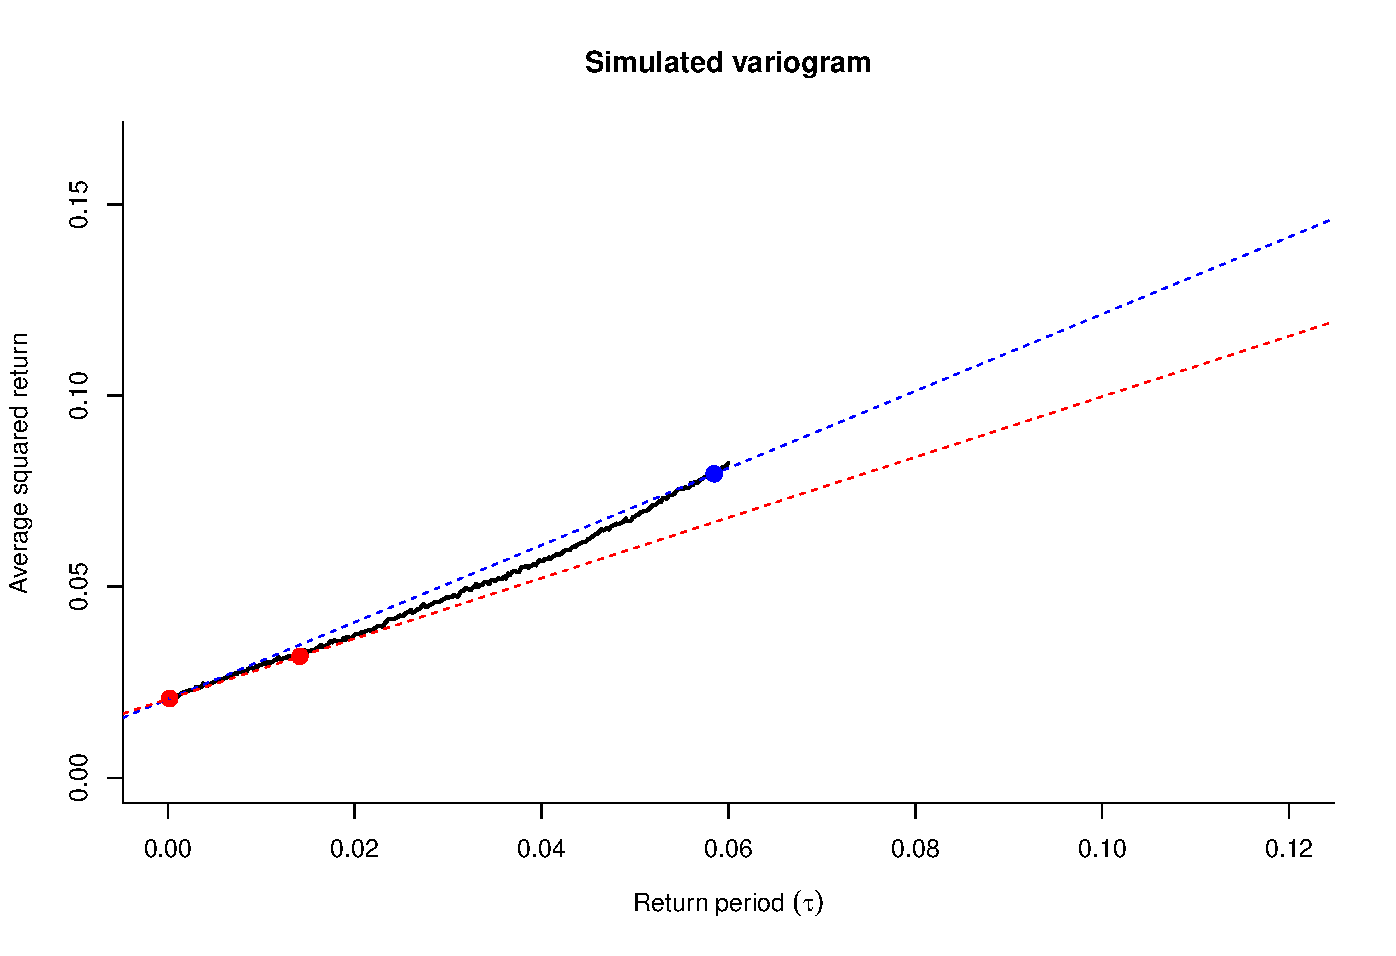
\includegraphics[width=\linewidth]{./Figures/simulatedVariogram.pdf}
\caption{\label{fig:simulatedVariogram} Simulated variogram from model (\ref{eq:model2}) with $\eta = 0.1$, $\sigma = 1$, $n = 5000$ and $\tau = k/n, k = 1,\dots, 300$.  Points are marked in red at $k =1, n^{1/2}$ and in blue at $n^{2/3}$.  Extrapolated values using the estimators of \citet{zhang2005tale} and \citet{zhang2006efficient} are indicated by the dashed lines in blue and red, respectively.}
\end{figure} 
The observations are assumed to be made at regularly spaced times $t_i = i/n, i= 0,\dots n$.
The objective is to estimate $v = \int^1_0 \sigma^2(s) ds = \EE [\breve{X}_n - \breve{X}_0]^2$.  
The variogram estimator is 
$$\hat{\Gamma}(k/n) = \frac{\sum_{i=k}^n[X(t_i) - X(t_{i-k})]^2}{n-k+1}, \quad k=1,\dots,n.$$
From (\ref{eq:variogramexp}) under the model (\ref{eq:model2}) we expect to see an approximately linear plot, with slope $v$.  To estimate the slope, two points can be chosen, say $1/n$ and $k/n$ and the slope estimated by
$$\hat{V} = \frac{\hat{\Gamma}(k/n) - \hat{\Gamma}(1/n)}{k/n - 1/n}.$$
One of the ways explaining, other methods of estimating volatility is trying to reproduce
this line which increases as return period increases to estimate the slope of the line. One
simple way to estimate the slope is to choose two points on the line on the variogram plot,
to estimate the slope from this two points, (two red dots).
This is essentially the two scale estimator considered by \citet{zhang2005tale}. 
The estimator is biased but the authors show that it is infill consistent when $k = k(n)$ is chosen to grow as  $n^{2/3}$, in which case the MSE (mean square error) of the estimator is of order $n^{-1/3}$. This is the  same order of convergence as the estimator in Section \ref{sec:infillconsistent}. 

\citet{zhang2006efficient} 
then goes on to consider an estimator that combines all of the values of $\hat{\Gamma}(k/n)$ up to $k \sim n^{1/2}$, effectively fitting a straight line through these values. She shows that the MSE of her `multiscale estimator' is or order $n^{-1/2}$. In an other word,
Zhang chooses several points along this variogram and combines them in the way to
fit a straight line through the variogram plot and uses the slope of the fitted line as the
volatility estimate.


The estimator proposed by \citet{jacod2009microstructure} can also be thought of as a variogram estimator, where the process $X$ is replaced by a moving average of $X$ over $k$ successive time points and the variogram is computed with these average values. They show that by choosing $k$ of order $n^{1/2}$ the MSE of their estimator is of order $n^{-1/2}$. This rate can be shown to be optimal when the volatility is constant.    
 
\subsection{Kernel methods}
In a series of papers \citet{barndorff2004regular,barndorff2008designing,barndorff2009realized} have developed a range of kernel-based volatility estimators.  These estimators are weighted linear combinations of the empirical autocovariances of the returns. They are directly related to the estimators of  \citet{zhang2005tale}, \citet{zhang2006efficient} and \citet{zhou1996high}.  For example, Zhou's first estimator (\ref{eq:Zhou1}) can be written as the linear combination $G = \hat{\gamma}_0 + \hat{\gamma}_1 + \hat{\gamma}_{-1}$ where
$$ \hat{\gamma}_h = \sum_{i=1}^n R_{i,1} R_{i+h,1},\quad h \in \mathbb{Z}.$$
Kernel based methods were originally developed in the classical problem of estimating the variance of $X$ from the observed values of a stationary sequence $X_1,\dots,X_n$ \citep{newey1987simple}. Barndorff-Nielsen et al.\ show that the asymptotic behaviour of simple kernel-based volatility estimator is strongly influenced by ``edge effects''. They show how to select kernel weightings to achieve the optimal order of infill asymptotics. The kernel weightings are applied to the autocovariances to form linear combinations of the autocovariances.  There is a connection to spectral density estimation and Fourier methods via the representation of the spectrum in terms of autocovariances.

\section{Observed price -- activity time}\label{sec:timedependency}
The modelling of time-varying volatility is important when the data are limited to prices at an arbitrary set of discrete times. For exchange traded assets, other measures of activity are known to be tied strongly to price fluctuations, as described previously in Section \ref{sec:timechange}.  There is now substantial evidence that volatility can be stabilised when measured on an `activity' time scale \citep{clark1973subordinated, ane2000order, griffin2008sampling}. Transaction time and `tick' time are common choices. Alternative measures of `activity' time are closely guarded intellectual property in the world of high-frequency algorithmic trading. 

The principal advantage of working on a volatility stabilised time scale is that simple recursive methods with constant coefficients based on the Kalman filter can be developed. Coefficients are determined by maximising empirical profitability in simulation, real-time application, or with historical data.  

Measuring volatility on a suitably modified time-scale provides a simple way of dealing with time-varying volatility. Switching clocks is a fundamental idea in finance. The
paradigm in the market is event-based time. As modifications of chronological time, a
clock should run as the same speed as trading activity that might be taking account of volume
traded or the actual activity on the order book. The standard inhomogeneous log-price model in physical time,
$$d\breve{X}(t) = \sigma(t) dB(t),$$  then 
has $ \sigma^2(t) = \psi(t) \beta^2,$
where $\psi(t)$ is the observed activity intensity at time $t$ and $\beta^2$ is a constant factor be estimated.  

If we let $s = \Psi(t) = \int_0^t \psi(u) du$ be the new time-scale and $\breve{Y}(s) = \breve{X}(t)$, then
$$d\breve{Y}(s) = \beta dB(s),$$
so the log-price process is transformed into Brownian motion with constant infinitesimal variance. The integrated variance over a period of time $(0,T)$ is then
$$ \int_0^1 \sigma^2(s) ds = \beta^2 \int_0^1 \psi(s) ds = \beta^2 \Psi(1),$$  
and as a result the assessment of integrated variance is reduced to the estimation of the constant parameter $\beta^2$. 

There is particular simplification when the activity clock is simply a count of activity events. Observation times on this clock are effectively successive integers. If the clock successfully stabilises the volatility, the returns of $\breve{X}_i$ have constant variance $\alpha^2$ and an estimate $\hat{\alpha}^2$ can be obtained by Zhou's subsampling method \eqref{eq:zhouGk}. The estimated integrated variance over the physical time interval $(0,1)$ is then $\hat{\alpha}^2$ multiplied by the number of activity events in $(0,1)$.

\subsection{Maximum likelihood and Kalman filter}
With a volatility stabilising clock, observations form a homogeneous ARIMA sequence, and the sequence of returns is MA[1].  In this framework, the problem simplifies to finding the MLEs of the parameters of a simple moving average sequence for which the Kalman filter is well adapted. In this formulation the asymptotic variance of the MLE of $\alpha^2$ is known to be of order $n^{-1/2}$, see \citet{ait2005often}. The convergence rate is very slow -- and it does not go to 0 rapidly as we would think. It is the noise that causes the problem.  Nevertheless, Kalman filter allows us to write down the
likelihood, to explore the likelihood space to maximize it.

Other authors have suggested \emph{pre-whitening} the sequence of returns by representing them in the form
$$ R_i = X_i - X_{i-1} = \breve{X}_i - \breve{X}_{i-1} + \epsilon_i - \epsilon_{i-1} = W_i - \theta W_{i-1},$$
where $(W_i)$ are iid $N(0,v_W)$ and the quantities $\theta$ and $v_W^2$ are given by the equations
\begin{align*}
\alpha^2 + 2\eta^2 &= (1-\theta^2)v_W^2\\
\eta^2 &= \theta v_W^2.
\end{align*} 
The \emph{pre-whitened} $(W_i)$ are then recovered by applying an EWMA to the sequence $(R_i)$. This approach is investigated by \citet{corsi2001consistent} who provide numerical comparisons of various volatility estimates based on these ideas.   

\section{Model criticism}
In this section we develop a Monte Carlo goodness-of-fit test for the standard model (\ref{eq:model2}). The test is aimed specifically at the assumptions underlying the volatility estimators in Section \ref{sec:longerreturns}. We apply the test in an empirical study of EBS data on the Euro/USdollar exchange rate between August 2008 and October 2009. 

The standard model (\ref{eq:model2}) has been criticised by various authors.  \citet{hansen2006realized} provide a very thorough analysis of the model assumptions, illustrating with data from 30 stocks in the Dow Jones Industrial Average.  Robustness to model specification is  emphasised by \citet{jacod2009microstructure} in their construction of pre-averaging estimators. 

Our test is based on the observation that under (\ref{eq:model2}) with  fixed $k \geqslant 1$ and $j \geqslant 1$, the collection of disjoint returns 
\begin{equation}\label{eq:disjointreturns} W_i = R_{ik +(i-1)j,k}, \quad i= 1,\dots,N,\end{equation}
are independently $N(0,\nu^2_i)$ with
\begin{align*}
\nu^2_i &= \int_{\tau_{i-1}}^{\tau_i} \sigma^2(s) ds + 2\eta^2 \\
\tau_i &= t_{ik+(i-1)j}, \quad i= 1,\dots,N,
\end{align*}
and $N = \lfloor (n+j)/(k+j)\rfloor$.         
It follows that 
$$ \sum_{i=1}^p W_i \overset{\text{distn}}{=} B\left(\sum_{i=1}^p \nu^2_i\right), \quad p = 1,\dots,N,$$
where $B(t),t>0$ is a standard Brownian process. 

In general, if a process has independent normally distributed increments then
by changing the time scale, it ends up as a Brownian motion observed at a sequence of times. 
Volatility is not constant, it
changes, and increments have different variances. That� is the assumption in this model. Therefore,
if we choose the correct time scale, we can convert this process into Brownian motion and
we can test whether that was correct by checking if it is consistent with Brownian motion
properties. One of the property is Brownian bridge. 

Suppose that 
$$S(t) \overset{\text{distn}}{=} B(\Psi(t)), \quad 0<t<T,$$
for an increasing function $\Psi$ then, by a time transformation,
$$ \tilde{B}(u) = \frac{S(\Psi^{-1}[u\Psi(T)]) - u S(T)}{\sqrt{\Psi(T)}}, \quad 0 <u<1$$
is a Brownian bridge.  To test whether $\Psi$ is the correct time transformation we can consider the maximum value of $|\tilde{B}(u)|$, as in the Kolmogorow-Smirnov test. 
Note that 
$$ \max_{0<u<1}\left|\frac{S\{\Psi^{-1}[u\Psi(T)]\} - u S(T)}{\sqrt{\Psi(T)}}\right| = \max_{0<t<T}\left|\frac{S(t) - S(T)\Psi(t)/\Psi(T)} {\sqrt{\Psi(T)}}\right|,$$
so the test rejects when the maximum value of  $S(t) - S(T)\Psi(t)/\Psi(T), 0<t<T$ exceeds some critical value.

For our test, we mimic this approach and use $T^* = \max_{p} |T_p|$ as a test statistic
where
\begin{equation}\label{eq:MCstatistic} T_p = \sum_{i=1}^p W_i -  \frac{\sum_{i=1}^p W^2_i}{\sum_{i=1}^N W^2_i} \sum_{i=1}^N W_i,\quad p = 1,\dots,N \end{equation}
and the terms $\sum_{i=1}^p W^2_i$ are used as a proxy for $\sum_{i=1}^p \nu_i^2.$

We want to see how often this trajectory deviates from the expected
trajectory and whether or not it is too far from where it is supposed to be.
We assess the significance of $T^*$ with a Monte Carlo p-value, independently randomising the sign of each $W_p, p=1,\dots,N$.  The observed value of $T^*$ is then compared with (say) 999 randomised values $T^*(m), m = 1,\dots,999$ to obtain the Monte Carlo p-value, in the usual manner -- see \citet{barnardMCtest}. 

\subsection*{Application to Euro/USdollar exchange rate}
Data for Euro/USdollar trades on EBS for the period August 2008 and October 2009 were made available by William Hooper of Xdirect. The Monte Carlo test was applied to each full trading day with four $(k,j)$ pairs and 999 Monte Carlo samples in each case. Histograms of the p-values are shown in Figure \ref{fig:MCtestChap}.
\begin{figure}[ht]
\centering
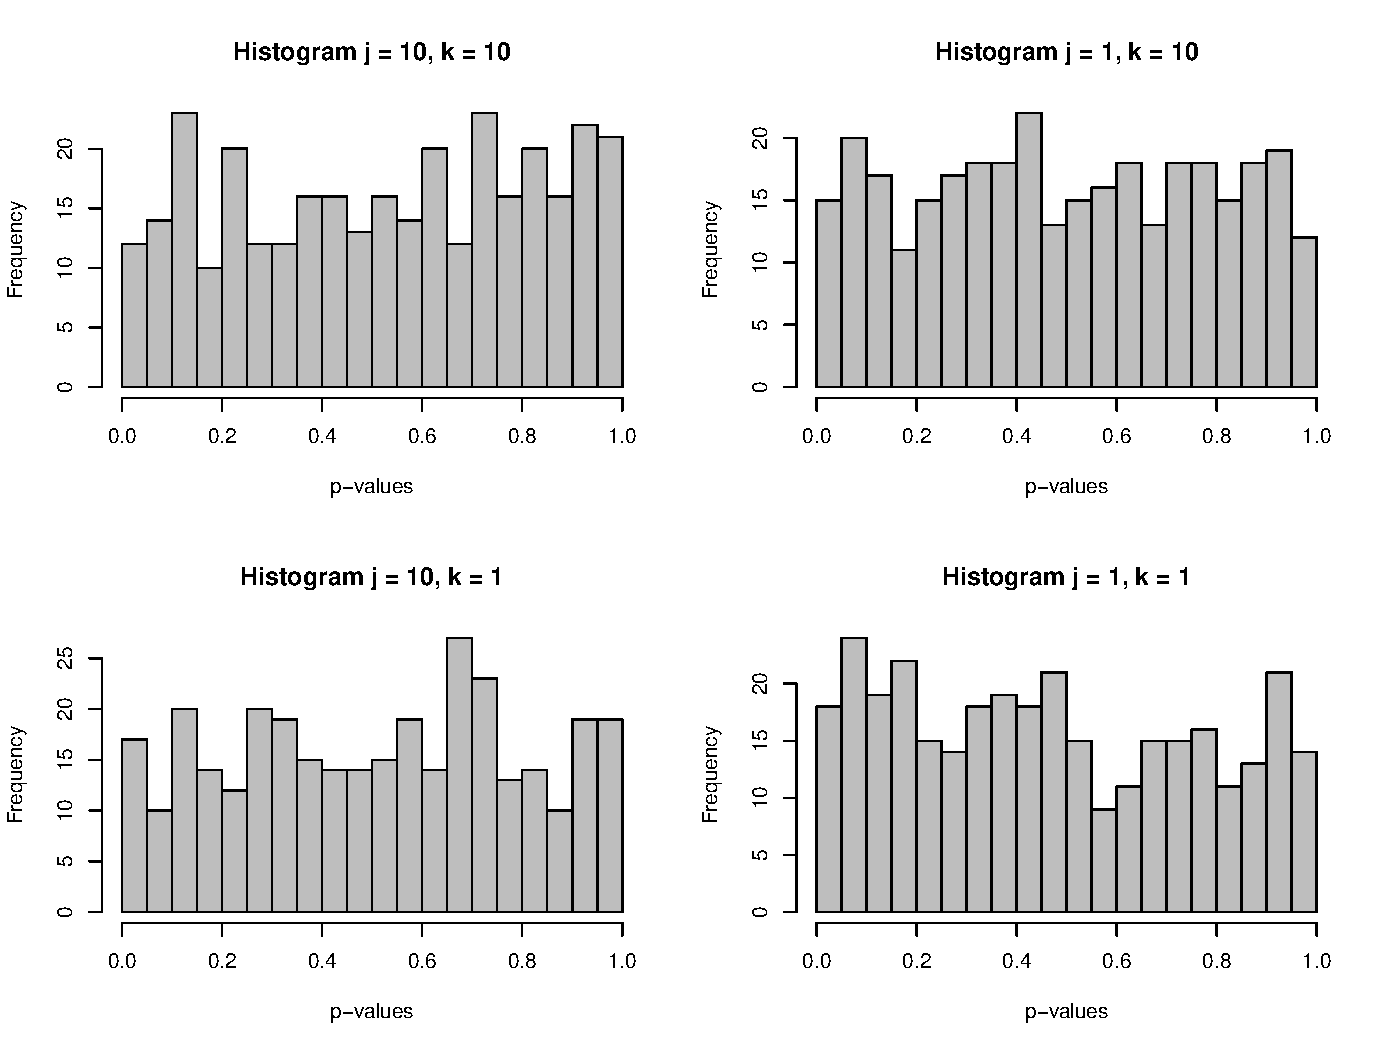
\includegraphics[width=\linewidth]{./Figures/MCtestChap3.pdf} 
\caption{\label{fig:MCtestChap}Monte Carlo p-values based on the test statistic (\ref{eq:MCstatistic}) where $\{W_i\}$ are defined in (\ref{eq:disjointreturns}). The data are tick-by-tick trade prices of Euro/USdollar transactions on the EBS exchange for 328 trading days between August 2008 and October 2009}
\end{figure}

As can be seen, the p-value distributions for all these $(k,j)$ pairs are relatively flat showing no reason to reject model (\ref{eq:model2}). See \citet{hansen2006realized} and Chapter 6 for further discussion.


\section{Robustness and volume effects}
The observed log-price in high-frequency data is commonly assumed to be a combination of the unobservable theoretically efficient log-price and some noise component $\epsilon$ due to the imperfections of the trading and recording process, the so-called {\it microstructure} of the market. Model \eqref{eq:model2} attempts to capture this structure. Less restrictively, we can think of the $\epsilon$ process as a combination of discretisation (i.e.\ rounding error) and independent random noise. When the bid/ask spread is small, the discretisation component will be dominant. More generally, the noise term will capture effects due to bid/ask bounce, targeted price reaction and trade and quote volume.  \citet{jacod2009microstructure} argue convincingly that their pre-averaging approach using smoothed values of the log-price data will provide estimators that are robust to model misspecification. Here we will see that stability can also be achieved by using prices derived from deeper levels of the order book. 
\subsection{Volume effects}
In this section, we will investigate the daily pattern of volatility in depth-dependent pricing of the US Dollar -- Japanese Yen exchange rate, making use of the estimator developed in Section \ref{sec:infillconsistent}. 

The data sets are the quote ladders in the EBS order book for USD--JPY foreign exchange. Observations are tick-by-tick with quotes every 100 milliseconds.  

As a first step, the \emph{regular prices} at each time, were determined for various depth of volume: 2, 5 and 10 million US dollars.  For example the regular ask price at 2 million dollars is the price in Yen per Dollar that is required to buy that amount of US currency.  The regular mid-price is then calculated as the geometric mean of the regular bid and ask prices.   By taking logarithms, these become $\{X_i\}$, the data to be processed.

The volatility was then estimated for each hour of each day in each month, using all tick-by-tick data.  The results were then averaged to produce the plots in Figure \ref{AugSepOct}.
 
\begin{figure}[!ht]
\centering
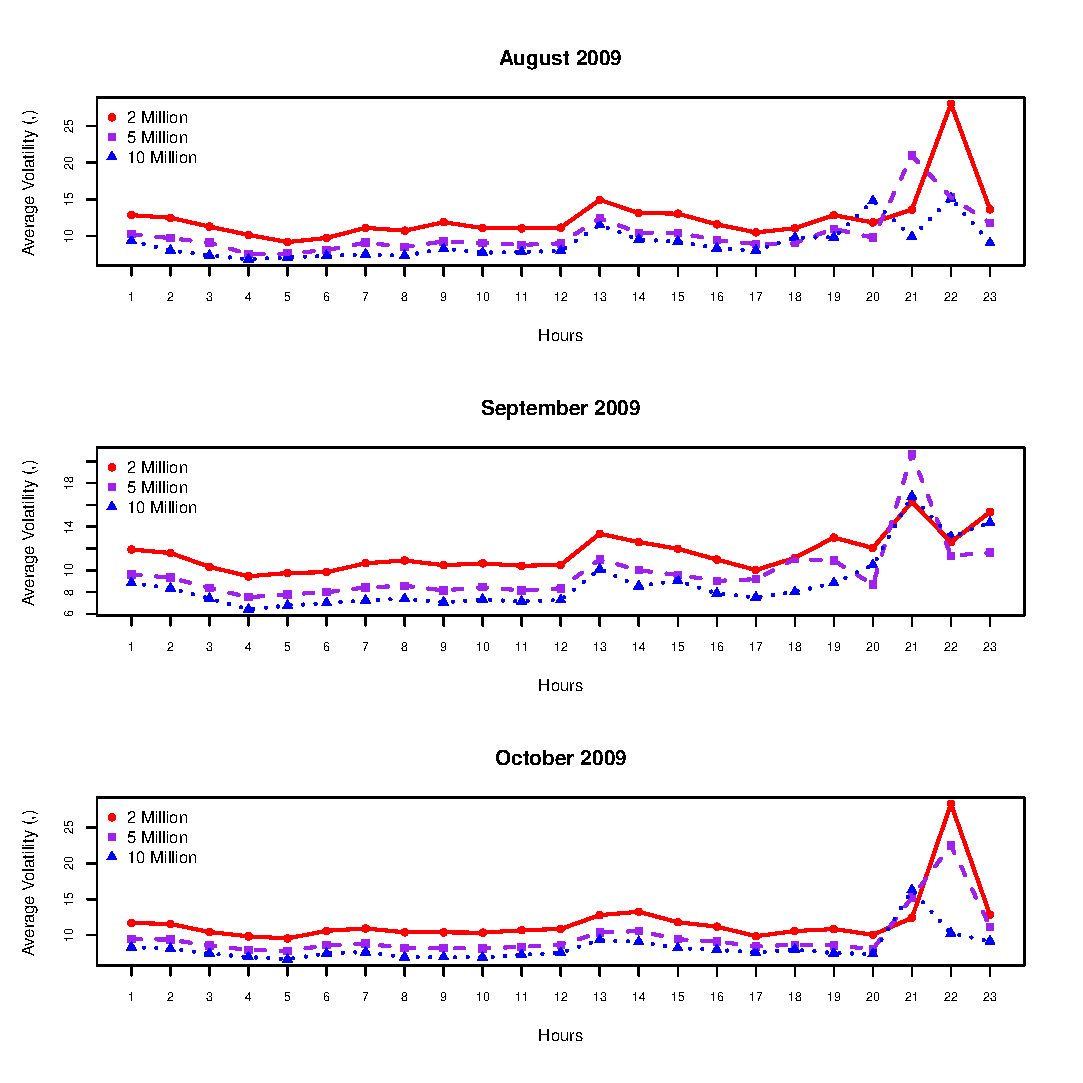
\includegraphics[width=\linewidth, height = 1.2\linewidth]{./Figures/augsepoct.eps}
\caption{USDJPY Hourly Average Volatility in August, September and October 2009 by using regular 
prices constructed from quote-by-quote prices of different volumes.\label{AugSepOct} }
\end{figure}
 
From the three figures we see immediately that volume-dependent volatility is highest in the concluding hours of each day, when trading is light. In such periods market makers are less active which has the effect of increasing the spread and as a result regular prices have to be found deeper into the order book.  Furthermore, there is a visible bump in each curve at around 1:30 PM each day, corresponding to the time at which important economic news items are usually announced.  This underlines the importance of identifying and taking account of points in time at which there are substantial price movements, predictable or otherwise. 

We observe that there is a consistent reduction in the volatility estimates when prices are calculated using an increasing proportion of the order book.  Interestingly we also find that the size of $\eta$, a measure of the microstructure effect,  is substantially smaller with these volume-dependent estimates of volatility compared with values calculated using the simple mid-price. 


